%!TEX root = ../Thesis.tex

\section{Sutskever}

The model in \autoref{sec:Long-Short-Term-Memory} - \nameref{sec:Long-Short-Term-Memory} provides an elegant way to classify each word in a sequence of text, this can be useful to classifying the mood of a word (positive, negative or neural) or similar cases where there is a one to one alignment between a word and a output class. This kind of problem is called sequence classification \cite[p.~10]{alexgraves}. However for finding a good latent representation for a document there dosen't exists such an alignment, thus sequence classification is not very useful.

The Sutskever model provides a method for finding a latent representation given some input document. Unfortunately this is a supervised model, as it also requires an output sequence. In the original paper \cite{sutskever} the model is used to translate english text to french text.

The overall idea is to have two neural networks, an encoder which takes an input document and outputs a vector, and a decoder which takes the same vector and outputs a document. The vector will then be a latent representation of the input document and hopefully this will contain enough information such that the document can be reconstructed in another language.

\begin{figure}[H]
	\centering
	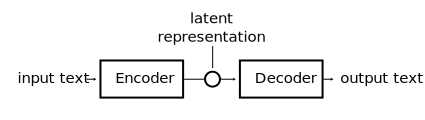
\includegraphics[scale=0.7]{theory/sutskever-overview}
	\caption{Rough overview of the Sutskever model.}
\end{figure}

In the case of news articles translations are quite rare, so instead the first paragraph is used as an input and the article title is used as an output. This way the latent representation will hopefully contain an encoded resume of the article.

\subsection{Text encoding}

The Sutskever paper \cite{sutskever} used a lot of computational resources (8 GPUS over 10 days) to manage the large network (8 layers with $1000$ LSTM units each) and a large softmax (output vocabulary was at 80000 words). Because Theano currently don't support using more than one GPU the network size is reduced and letters are used instead of words.

Using letters instead of words means that the sequences gets longer. The avenge word length in english text is 5.1 character, including the space separator one should expect 6.1 longer sequences. However by using letters the softmax size is decreased from 80000 words to just 78 letters. It should be noted that Unicode NFKD normalization \cite{unicode-normalization} was used to remove accents and ligatur, rarely used letters was also removed to reduce the softmax size further.

The Sutskever paper \cite{sutskever} do indicates that the model may not work for long sequences, which could be a problem when using letters instead of words. However given the limited resources this still seams like a good solution.

The input and output sequence are both encoded using 1-of-V encoding where V is the amount of unique letters. In order to indicate to the network when an input or output sequence is ended an end-of-sequence ``letter'' is added to the vocabulary. This special letter will be denoted \texttt{<eos>}.

\todo[inline]{The paper also reverses the output sequence.}

\subsection{Forward pass}

The encoder works like a normal LSTM network except that the network output $y_k^{t_e}$ isn't used \todo{The notation is not introduced explicitly}. The network is just used to scan though the input sequence $x^{t_e}$ and the network state is completely carried by the hidden output $b_{h_\ell}^t$ and the cell state $s_{c_\ell}^t$. When the network receives an \texttt{<eos>} letter, the hidden output and the cell state from the last layer is used as the latent representation.

\begin{figure}[H]
	\centering
	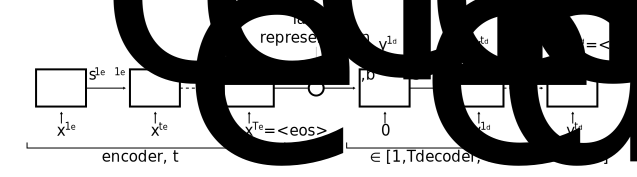
\includegraphics[scale=0.75]{theory/sutskever-notation}
	\caption{Each box represent a single time iteration.}
\end{figure}

The latent representation consisting of the hidden output $b_{h_{L}}^{T_e}$ and cell state $s_{c_{L}}^{T_e}$ is then used to initialize the hidden output and cell sate in the decodes first layer.

\begin{equation}
\begin{aligned}
b_{h_1}^{0_d} &= b_{h_{L}}^{T_e} \\
s_{c_1}^{0_d} &= s_{c_{L}}^{T_e}
\end{aligned}
\end{equation}

The decoder is more special than the encoder, because the network output $y_k^{t_d}$ is used as the input in the next time iteration. For initializing the decoder input $y_k^{0_d} = 0$ is used.
\begin{equation}
x^{t_d} = y_k^{t_d - 1}, \quad \text{where: } y_k^{0_d} = 0
\end{equation}

The $y_k^{t_d}$ sequence is the output sequence and is compared to the target sequence using a normal entropy loss function.
\begin{equation}
\mathcal{L} = - \sum_{t_d}^{T_d} \sum_{k}^K t_k^t \ln(y_k^{t_d})
\end{equation}

In practice where mini-batch gradient decent is used for optimization, the output and target sequences for all observations in the mini-batch, must be equally long to fit the datastructure. To do this the taget sequence is padded with \texttt{<eos>} letters, until it fits the max sequence length in the mini-batch. This means that the network doesn't stop predicting at the first \texttt{<eos>} output letter, but continues until the max sequence  length in the mini-batch is meet. A side effect of this is that the loss function will punish non-\texttt{<eos>} letters after the first $\texttt{<eos>}$ letter. However because it should be fairly easy for the network to learn $y_k^{t_d} = \texttt{<eos>} \Rightarrow y_k^{t_d+1} = \texttt{<eos>}$, this side effect shouldn't matter that much.

The backward pass will look somewhat similar to the simple LSTM network (see section \ref{sec:theory:lstm:backward-pass}), however it will be much more complicated because the entire sutskever network actually consists of two somewhat separate networks. For this reason the deriving the backward pass have been skipped here. In practice Theano \cite{theano-a, theano-b} is used to derive the backward pass.
